\documentclass[letterpaper, 12pt]{article}
\usepackage[francais]{babel}

\usepackage{amsmath,amsfonts,amsthm,amssymb, graphicx,wasysym,multirow}
\usepackage[latin1]{inputenc}

\pagestyle{plain}

\setlength{\topmargin}{-2cm}
\setlength{\textheight}{23.5cm}
\setlength{\textwidth}{18cm}
\setlength{\oddsidemargin}{-1cm}
\setlength{\parindent}{0pt}

%\pdfoutput=1


\begin{document}


1-- Which of these are factors of 72 written in prime numbers?\\
a$)$ $2 \times 4 \times 9$\\
b$)$ $2 \times 6^{2}$\\
c$)$ $2 \times 6^{6}$\\
d$)$ $2^{3} \times 3^{2}$\\

Answer: d$)$\\

Explanation:\\
$2 \times 4 \times 9 = 72$, but 4 and 9 are not prime numbers.\\
$2 \times 6^{2} = 2 \times 6 \times 6 = 72$, but 6 is not a prime number.\\
$2 \times 6^{6} = 2 \times 6 \times 6 \times 6 \times 6 \times 6
\times 6 = 93\,312 \neq72$.  Again,\\ 6 is not a prime number. Thus, the correct answer is d).\\



11-- Obelix goes to the grocery store. He buys 480\,g of ground beef at 8.56 per kg, two bags of carrots for 1.99 each and three peppers for 99 cents each. Which order of operations allows us to calculate the total amount of this transaction.?\\
a) $0,48 \times 8,56 + 2 \times 1,99 + 3 \times 99$\\
b) $0,48 \times 8,56 + 2 \times 1,99 + 3 \times 0,99$\\
c) $480 \times 8,56 + 2 \times 1,99 + 3 \times 0,99$\\
d) $480 \times 8,56 + 2 \times 1,99 + 3 \times 99$\\

Answer: b)\\

Explanation:\\
One must not forget to convert 480\,g into 0,48\,kg and 99 cents to 0.99. Here is an example of a correct order of operations:  $0,48 \times 8,56 + 2 \times 1,99 + 3 \times
0,99$.\\
Thus, the correct answer is b).\\

12-- Which of the following statements is true?\\
a) $\frac{3}{10}=0,3=3\times10^{0}$ \\ [2mm]
b) $\frac{3}{10}=0,03=3\times10^{-1}$ \\[2mm]
c) $\frac{3}{10}=0,3=3\times10^{-1}$ \\[2mm]
d) $\frac{3}{10}=0,03=3\times10^{0}$ \\

R\'eponse : c)\\

R\'etroaction :\\[2mm]
In $\frac{3}{10}=0,3=3\times10^{0}$, the false value is
$3\times10^{0}=3$.\\[2mm]
In $\frac{3}{10}=0,03=3\times10^{-1}$, the false value is 0,03.\\[2mm]
In $\frac{3}{10}=0,03=3\times10^{0}$, all the values are different.\\[2mm]
The answer is c).\\



21-- Which is the smallest out of the four following numbers?\\
a) $\frac{1}{5}$\\
b) $\left( \frac{2}{7}\right)^{2}$\\
c) $\left( \frac{1}{3}\right)^{3}$\\
d) $\left( \frac{3}{4}\right)^{2}$\\

Answer: c)\\

Explanation:\\
$\frac{1}{5}=0,2\\
\left( \frac{3}{4}\right)^{2}=0,5625\\
\left( \frac{1}{3}\right)^{3}=0,\overline{037}\\
\left(\frac{2}{7}\right)^{2}=0,081\,632\,65\ldots\\

The correct answer is c).\\



31-- Which symbol represents all rational numbers?\\
a) $\mathbb{N}$\\
b) $\mathbb{Q}$\\
c) $\mathbb{R}$\\
d) $\mathbb{Z}$\\

Answer: b)\\

Explanation:\\
$\mathbb{N}$ represents natural numbers.\\
$\mathbb{Q}$ represents rational numbers.\\
$\mathbb{R}$ represents real numbers.\\
$\mathbb{Z}$ represents whole numbers.\\
Thus, the correct answer is b).\\


41-- Which of these numbers is the LCM (Least Common Multiple) of
$2^{2}\times3^{4}\times5\times7^{2}$ and $2\times3^{5}\times7^{3}\times11$?\\
a) $2\times3\times5\times7\times11$\\
b) $2\times3^{4}\times7^{2}$\\
c) $2^{2}\times3^{5}\times5\times7^{3}\times11$\\
d) $2^{3}\times3^{9}\times5\times7^{5}\times11$\\

Answer: c)\\

Explanation:\\
One must compare the exponents of each prime factor in each number and choose the smallest of the two. Next, prime factors affected by the chosen exponents must be multiplied. The correct answer is c).\\


51-- Among the four numbers here below, which value of $y$ completes the following:
$252\div y=4$?\\
a) $y= \frac{4}{252}$\\[2mm]
b) $y= 4$\\[2mm]
c) $y= 63$\\[2mm]
d) $y= 1008$\\

Answer:  c)\\

Explanation:\\
The following proportions must be used: \\[2mm]
$\frac{252}{y}=\frac{4}{1}$, or $y = 252\times1\div4=63$. The correct answer is c).\\


61-- Which of the following numbers is a prime number?\\
a) 57\\
b) 59\\
c) 63\\
d) 81\\

Answer: b)\\

Explanation:\\
A prime number only has two divisors, 1 and itself. One must remember that 1 is not a prime number even if its only divisors are 1 and itself. Composite numbers are numbers that have more than two factors.\\
$19\times3 = 57\\
7\times9 = 63\\
9\times9 = 81$\\
57, 63 and 81 are all composite numbers. Thus, the correct answer is b).\\



71-- Among the following four choices, which one regulates multiplication signs?\\
a) $+\times+=+, \qquad+\times-=-,\qquad-\times+=-, \qquad-\times-=+$\\
b) $+\times+=+, \qquad+\times-=+,\qquad-\times+=+, \qquad-\times-=-$\\
c) $+\times+=+, \qquad+\times-=-,\qquad-\times+=-, \qquad-\times-=-$\\
d) $+\times+=+, \qquad+\times-=+,\qquad-\times+=-, \qquad-\times-=+$\\

Answer: a)\\

Explanation:  \\
The multiplication signs rule is given by:
\qquad+\times-=-,\qquad-\times+=-, \qquad-\times-=+$.\\
The correct answer is a).\\



81-- Among the following four choices, which one regulates division signs?\\
a) $+\div+=+, \qquad+\div-=-,\qquad-\div+=-, \qquad-\div-=+$\\
b) $+\div+=+, \qquad+\div-=+,\qquad-\div+=+, \qquad-\div-=-$\\
c) $+\div+=+, \qquad+\div-=-,\qquad-\div+=-, \qquad-\div-=-$\\
d) $+\div+=+, \qquad+\div-=+,\qquad-\div+=-, \qquad-\div-=+$\\

Answer: a)\\

Explanation:  \\
Division sign rules are given by:\\
$+\div+=+, \qquad+\div-=-,\qquad-\div+=-, \qquad-\div-=+$.\\
The correct answer is a).\\



91-- Mathexpert City's clock sounds every hour.  It sounds once at 1 a.m. and 1 p.m., twice at 2 a.m. and 2 p.m. $\ldots$ and twelve times at noon and midnight. Also, it strikes twice every hour at half-past the hour (or, at 1:30, 2:30, 3:30 \ldots) How many times per day does Mathexpert City's clock sound?\\

Answer: 204\\

Explanation: \\
On the hour, the clock sounds\\
$1+2+3+4+5+6+7+8+9+10+11+12+1+2+3+4+5+6+7+8+9+10+11+12=156$ times.\\
Furthermore, the clock sounds $24\times2=48$~times on the half-hour of every hour.\\
All together, the clock sounds a total of $156+48=204$ times.\\
The correct answer is 204.\\



101-- In each rectangular triangle, what is the sum of the acute angles?\\
a) 35$^{\circ}$\\
b) 45$^{\circ}$\\
c) 60$^{\circ}$\\
d) 90$^{\circ}$\\

Answer: d)\\

Explanation:\\
In a rectangular triangle, there is a straight angle measuring 90$^{\circ}$. Since the sum of interior angles is 180$^{\circ}$ and $180^{\circ}-90^{\circ} = 90^{\circ}$, there are 90 degrees left for the two other angles. The correct answer is d).\\

111-- How many extremities are there in a straight angle?\\

Answer: 0\\

Explanation: \\
A straight angle goes on to infinity on both sides. There are no extremities to it.  Thus, the correct answer is 0.\\


121-- Amongst the following elements, which one is essential for forming a translation?\\
a) An angle\\
b) A centre\\
c) A growing factor\\
d) An arrow\\

Answer: d)\\

Explanation:\\
Arrows contain all the essential information for a translation. They indicate the direction and distance for any displacement of the original figure. The correct answer is d).\\



131-- Which of the following characteristics is typical of a trapezoid?\\

a) A pair of congruent sides\\
b) A pair of parallel sides\\
c) A pair of perpendicular sides\\
d) Two pairs of parallel sides\\

Answer: b)\\

Explanation:\\
   \begin{center}
    \includegraphics[height=3.39cm]{131.eps}
% napperon.eps : 300dpi, width=3.39cm, height=3.39cm, bb=0 0 400 400
    \end{center}
A trapezoid always has a pair of parallel sides. The correct answer is b).\\

132-- Of the following characteristics, which one is that of a parallelogram?\\

a) A single set of parallel sides.\\
b) Only two congruent sides.\\
c) Two sets of parallel sides.\\
d) Four congruent sides.\\

Answer: c)\\

Explanation: \\
   \begin{center}
    \includegraphics[height=3.39cm]{132.eps}
% napperon.eps : 300dpi, width=3.39cm, height=3.39cm, bb=0 0 400 400
    \end{center}
A parallelogram always has two sets of parallel sides.\\  The correct answer is c).\\


141-- How are sizes illustrated in a pictogram?\\
a) With bands.\\
b) With a broken line.\\
c) With picture patterns.\\
d) With dots.\\

Answer: c)\\

Explanation: \\
In a pictogram, drawings called picture patterns represent different sizes. The correct answer is c).\\


151-- A leak in Joe's hot water tank spills out 2 ml every 45 minutes, from Jack's 1 ml every 30 minutes, from Averel's 1.5 ml per 20 minutes and from William's 3 ml per hour. Which water tank leaks out the most hot water?\\
a) Averel's.\\
b) Jack's.\\
c) Joe's.\\
d) William's.\\

Answer: a)\\

Explanation:\\
The amount of water that each tank spills out during the same period of time must be compared to find this answer.\\

For 3 hours or 180 minutes: \\
Joe's tank:
$\frac{2\textrm{\,ml}}{45\textrm{\,min}}\times180$\,min =
2\,ml\,$\times$\,4 = 8\,ml\\ [2mm] Jack's tank:
$\frac{1\textrm{\,ml}}{30\textrm{\,min}}\times180$\,min =
1\,ml\,$\times$\,6 = 6\,ml\\ [2mm]
Averel's tank: $\frac{1,5\textrm{\,ml}}{20\textrm{\,min}}\times180$
\,min = 1,5\,ml\,$\times$\,9 = 13,5\,ml\\[2mm]
William's tank: $\frac{3\textrm{\,ml}}{60\textrm{\,min}}\times180$
\,min = 3\,ml\,$\times$\,3 = 9\,ml\\[2mm]
Thus, it is Averel's tank that leaks the most. The correct answer is a).\\


161-- Pumbaa travels 8 km in 60 minutes, Pocahontas 4.5 km in 30 minutes, Quasimodo 2 km in 20 minutes, and Esmeralda 1.75 km in 15 minutes. Who runs the fastest?\\

a) Esmeralda\\
b) Pocahontas\\
c) Pumbaa\\
d) Quasimodo\\

Answer: b)\\

Explanation:\\
One must compare distances traveled for the same period of time, for example 60 minutes. \\
Pumbaa runs 8 km in 60 minutes.\\
Pocahontas runs 9 km in 60 minutes.\\
Quasimodo runs 6 km in 60 minutes.\\
Esmeralda runs 7 km in 60 minutes.\\
Thus, Pocahontas runs the fastest. The correct answer is b).\\


171-- Which of the following fractions does not belong in the same group $\frac{39}{65}$, $\frac{3}{5}$, $60\,\%$ et 0,06,?\\

a) $\frac{39}{65}$\\[2mm]
b) $\frac{3}{5}$\\[2mm]
c) $60\,\%$\\[2mm]
d) 0,06\\

Answer: d)\\

Explanation:\\
Each expression is equal to 0.6 except 0.06. Thus, the fraction does not belong is 0.06. The correct answer is d).\\



181-- Bianca Castafiore's bird flew and went over to perch on a wooden post in the middle of the neighbor's pond. Castafiore cannot go and retreive her bird without knowing the depth of the pond. However, the neighbor told her that at the time that he planted the post in the bottom of the pond, half of the post was driven into the mud. Furthermore, he told her that a third of the post was under water, between the muddy bottom and the surface. Lastly, we know that the post sticks out 50 cm from the water's surface. What is the depth of the pond?\\

a) 50 cm\\
b) 100 cm\\
c) 150 cm\\
d) 200 cm\\

Answer: b)\\

Explanation: \\
We know that half of the post is in the mud, a third is under water and that the post sticks out 50 cm above the water's surface.\\[2mm]
$p$ represents the length of the post in cm.\\[2mm]
We know that $\frac{1}{2}p+\frac{1}{3}p+50$\,cm$\,=p$\\[2mm]
$\frac{3}{6}p+\frac{2}{6}p+50$\,cm$\,=p$\\[2mm]
$\frac{5}{6}p+50$\,cm$\,=p$\\[2mm]
50\,cm\,=\,$\frac{1}{6}p$\\[2mm]
300\,cm\,=\,$p$\\[2mm]
The post is 300 cm long. A third of the length is equal to the water's depth.\\
Thus, $\frac{1}{3}$ of 300\,cm is $\frac{1}{3}\times300$\,cm $=100$\,cm.\\
The pond is 100\,cm deep. Thus, the correct answer is b).\\


201-- What number comes next in the following sequence: 3, 5, 9, 15, 23, \ldots?\\

Answer: 33\\

Explanation: \\
This sequence's pattern is made up by adding + 2, + 4, + 6, + 8, + 10, \ldots\\
One must add 10 to come up with the term following 23.  \\
Since 23 + 10 = 33, the answer is 33.\\


211-- Which of the four equalities below is true if $a\neq 0$?\\
a) $\frac{1}{a}\times a = -1$\\[2mm]
b) $\frac{1}{a}\times a =0$\\[2mm]
c) $\frac{1}{a}\times a=1$\\[2mm]
d) $\frac{1}{a}\times a = a$\\

Answer: c)\\

Explanation: \\
When fractions are multiplied, the numerators are multiplied together and the denominators are multiplied together.  \\
$\frac{1}{a}\times a = \frac{1}{a} \times \frac {a}{1} = \frac{1\times
a}{a\times 1}=\frac{a}{a}=1$\\
Thus, the correct answer is c).\\




221-- What is the average price per CD for the four CD's that Lucky Luke bought given that he paid $b\,\$$ for the first, $c\,\$$ for the second, $r\,\$$ for the third and $s\,\$$ for the fourth?\\
a) $b+c+r+s \div4$\\
b) $\left( b+c+r+s\right) \div 4$\\
c) $4\div \left( b+c+r+s\right) $\\
d) $4\div b+c+r+s$\\

Answer: b)\\

Explanation:\\
To find the average price, one must first add up the sum of what was spent and then divide by the number of articles purchased. \\
$\left( b+c+r+s\right) \div 4$\\
The correct answer is b).\\


231-- Cleopatra's father is three years younger than Cleopatra's age quadrupled. In addition, the sum of their ages is 52. How old is Cleopatra's father?\\

Answer: 41\\

Explanation: \\
\
Let's say that\\
$C$ = Cleopatra's age;\\
$P$ = her father's age.\\

Now we have the two following equations:\\
$P = 4C -3\qquad$ (equation 1)\\
$P + C = 52 \qquad$ (equation 2)\\

By manipulating equation 2, we get\\
$P = 52 - C\qquad$  (equation 3).\\
Then we replace $P$ from equation 1 with its valued obtained in equation 3.
And now we get\\
$52\,-\,C\,=\,4C\,-\,3$.\\
$55\,=\,5C$\\
By dividing each equal part by 5, we reach\\
$11\,=\,C$.\\

Thus, $P=52-C=52-11=41$.\\
The correct answer is 41 years old.\\


241-- Which of the following expressions gives the circonference of a radius of a circle $r$?\\

a) $\pi r^{2}$ \\
b) 2$\pi r$ \\
c) 2$\pi r^{2}$ \\
d) 4$\pi r$ \\

Answer: b)\\

Explanation:\\
The circonference of a radius of a circle $r$ is 2$\pi r$.  The correct answer is b).\\


251-- On a Cartesian map, what is the name of the vertical axis?\\

a) Abscissa axis\\
b) Axis of rotation\\
c) Reflectional axis\\
d) Symetrical axis\\

Answer: b)\\

Explanation:\\
On a Cartesian map, the vertical axis is also the axis of rotation. The correct answer is b).\\



261-- Which of the following four choices lists off elements allowing us to completely define a homothetic transformation?\\

a) Two images\\
b) Two points\\
c) Two points and their image\\
d) The center and an image point\\

Answer: c)\\

Explanation: \\
To define a homothetic transformation, one needs two points and their image because this allows us to find the center of the homothecy. To do this, one only needs to draw a straight line through a point and its image for each of the two pairs of points. The intersection of the two straight lines becomes the center of the homothecy. With the center, it is now possible to identify the homothetic relation. The correct answer is c).\\



271-- Which of the following four statements is true?\\

a) When a homothetic relation is positive, the final figure is greater than the initial figure.\\
b) When a homothetic relation greater than 1 or less than $-1$, the final figure is larger than the initial figure.\\
c) When a homothetic relation is greater than 1 or $-1$, the final figure is greater than the initial figure.\\
d) When a homothetic relation is only greater than 1, the final figure is greater than the initial figure.\\

Answer: b)\\

Explanation: \\
For the final figure to be greater than the initial figure, the homothetic relation must be greater than 1 or less than $-1$.
Thus, the correct answer is b).\\



281-- Which of the following portrays a Cartesian map translation?\\

a) $t_{\left( a,\,b\right) } :\left( x,\,y\right) \longmapsto \left( x\times
a,\,y\times b\right) $\\
b) $t_{\left( a,\,b\right) } :\left(x,\,y\right)\longmapsto
\left(x+a,\,y+b\right) $\\
c) $t_{\left( a,\,b\right) } :\left(x,\,y\right)\longmapsto \left(x\div
a,\,y\div b\right) $\\
d) $t_{\left( a,\,b\right) } :\left(x,\,y\right)\longmapsto \left(x\times
a,\,y\div b\right) $\\

Answer: b)\\

Explanation:\\
A translation is represented by $t_{\left( a,\,b\right) }
:\left(x,\,y\right)\longmapsto \left(x+a,\,y+b\right)$.  The correct answer is b).\\



301-- In figure skating, in 1988, Japan's Midori Ito was the first woman to execute a triple axel. This means that the skater spun around three and a half times in mid-air. Among the following choices, which one represents the number of degrees that she spun around in the air?\\
a) $720^{\circ}$\\
b) $900^{\circ}$\\
c) $1260^{\circ}$\\
d) $1440^{\circ}$\\

Answer: c)\\

Explanation: \\
One spin equals 360$^{\circ}$ and a half spin equals 180$^{\circ}$.
So, three and half spins equal 360$^{\circ}$ + 360$^{\circ}$ +
360$^{\circ}$ + 180$^{\circ}$ = 1260$^{\circ}$.\\
The correct answer is c).\\


311-- The circonference of the front wheel on Tarzan's bicycle is
188,50\,cm.  The radius of the front wheel of Eureka's bicycle is
25 cm.  Which of the following statements is true?\\

a) The front wheel on Tarzan's and Eureka's bicycle are the same size.\\
b) The front wheel on Eureka's bicycle is the biggest.\\
c) The front wheel on Tarzan's bicycle is the biggest.\\
d) The front wheel on Tarzan's bicycle is the smallest.\\

Answer: c)\\

Explanation:\\
\
$C=2\pi r$\\[2mm]
We are looking for the radius of the front wheel of Tarzan's bicycle.\\[2mm]
$r=\frac{C}{2\pi}=\frac{188,50\textrm{\,cm}}{2\pi}=30$\,cm\\[2mm]
The front wheel on Tarzan's bicycle has a radius of 30 cm and on Eureka's has a radius of 25 cm.
The front wheel on Tarzan's bicycle is bigger than the radius on Eureka's bicycle.
The correct answer is c).\\



321-- The average of five numbers is 12.  If 10 is added to each of these five numbers, what is the new average?\\

a) The average remains at 12.\\
b) The new average is 14.\\
c) The new average is 17.\\
d) The new average is 22.\\

Answer: d)\\

Explanation:\\
Since the original average increases by 10, adding 10 to each number,  makes new average 22.
Thus, the correct answer is d).\\


331-- A postal code is formed by the following: a letter, a number, a letter, a number, a letter, and a number.
How many different postal codes is it possible to form with three letters and three numbers?\\

a) 108\\
b) $17\,576$\\
c) $12\,812\,904$\\
d) $17\,576\,000$\\

Answer: d)\\

Explanation: \\
One must consider the multiplication rule.  Then one must determine the number of possibilities for each step:\\
First step: 26 possibilities (26 letters in the alphabet).\\
Second step: 10 possibilities (10 numbers: 0, 1, 2, 3, 4, 5,
6, 7, 8 and 9).\\
Third step: 26 possibilities (26 letters in the alphabet).\\
Fourth step: 10 possibilities (10 numbers: 0, 1, 2, 3, 4,5,
6, 7, 8 and 9).\\
Fifth step: 26 possibilities (26 letters in the alphabet).\\
Sixth step: 10 possibilities (10 numbers: 0, 1, 2, 3, 4, 5,
6, 7, 8 et 9).\\
The multiplication rule states that one must multiply the number of possibilities at each step.\\
$26\times10\times26\times10\times26\times10=17\,576\,000$\\
Thus, the correct answer is d).\\



341-- In the 6/49 Lottery, Alfa Bettyicalorder chose numbers 1, 2, 3, 4, 5, 6.
Panoramix, on the other hand, chose the numbers, 3, 12, 26, 33, 37, and 42.
Which of the following statements is true?\\

a) Alphie Bettyicalorder has a better chance of winning the jackpot than Panoramix.\\
b) Alphie Bettyicalorder has just as good a chance as Panoramix of winning the jackpot.\\
c) Panoramix has a better chance of winning the jackpot than Alphie Bettyicalorder.\\
d) Panoramix has less of a chance of winning the jackpot than Alphie Bettyicalorder.\\

Answer: b)\\

Explanation: \\
In the 6/49 Lottery, every number combination has the same chances of winning the jackpot.
Thus, the correct answer is b).\\




351-- Which of the following four statements here below is true?\\
a) There is no decimal number between 0.37 and 0.38.\\
b) There is an infinite number of decimals between 0.37 and 0.38\\
c) There are 10 decimal numbers between 0.37 and 0.38.\\
d) There are 100 decimal numbers between 0.37 and 0.38\\

Answer: b)\\

Explanation:\\
There is an infinite number of decimals between 0.37 and 0.38.
For example, 0.3711 and 0.3713 are both located between 0.37 and 0.38.
The correct answer is b).\\


361-- Which of the four following equivalents is true?\\

a) $m^{1}=\frac{1}{m}$\\[2mm]
b) $m^{1}=1$\\[2mm]
c) $m^{1}=\sqrt{m}$\\[2mm]
d) $m^{1}=m$ \\

Answer: d)\\

Explanation: \\
The only correct equivalent is $m^{1}=m$.  The correct answer is d).\\


371-- If $x\neq0$, which of the following choices below is true?\\

a) $\frac{x^{a}}{x^{b}}=x^{a+b}$\\[2mm]
b) $\frac{x^{a}}{x^{b}}=x^{a-b}$\\[2mm]
c) $\frac{x^{a}}{x^{b}}=x^{a\cdot b}$\\[2mm]
d) $\frac{x^{a}}{x^{b}}=x^{a\div b}$\\

Answer: b)\\

Explanation: \\
The statement $\frac{x^{a}}{x^{b}}=x^{a-b}$
expresses one of the correct property of exponents.
The correct answer is b).\\


381-- What powers are used in scientific notation?\\

Answer: 10\\

Explanation: \\
Scientific notation uses powers of 10.\\


391-- Among the four choices below, which one is a term similar to
$4v^{3}t^{2}$?\\

a) $v^{3}t^{2}$\\
b) $v^{1}t^{4}$\\
c) $4v^{5}$\\
d) $4t^{5}$\\

Answer: a)\\

Explanation: \\
A term similar to $4v^{3}t^{2}$ is a term in the form of $cv^{3}t^{2}$,
where $c$ is a random number called a coefficient.
Thus, the correct answer is a).\\



401-- Out of the following four choices, which one is the product of $-7$ and $5\alpha-4$?\\

a) $7\alpha$\\
b) $-7\alpha$\\
c) $-35\alpha-28$\\
d) $-35\alpha+28$\\

Answer: d) \\

Explanation: \\
$-7$ is distributed to $5\alpha$ and $-4$.
Thus, the correct answer is d).\\




411-- Nestor invites several friends to his house and wants to offer them two kinds of juice when they come over: apple juice and fruit punch. So, he buys 10 cans of frozen juice. How many cans of apple juice did he buy given that he bought four times more apple juice than fruit punch? \\

Answer:  8\\

Explanation: \\
Let's say\\
$P$ = number of apple juice cans;\\
$F$ = number of fruit punch cans.\\
$P+F=10 \qquad $(equation 1)\\
$P=4F \qquad$ (equation 2)\\
$P$ is replaced from equation 1 with its value calculated in equation 2.
We get $4F+F=10$.\\
$5F=10\\
F=2$\\
F's value is replaced in equation 1 and we get $P+2=10$.\\
$P=8$\\
Nestor bought 8 cans of apple juice.\\



421-- Among the four choices here below, which one completes correctly the following table?\\
\begin{tabular}{|c|c|} \hline

{\bf X-coordinate ($x$)} & {\bf Y-coordinate ($y$)}  \\ \hline \hline
1 & 0 \\ \hline
2 & 3 \\ \hline
3 & 8 \\ \hline
4 & 15 \\ \hline
5 & 24 \\ \hline
$\ldots$ & $\ldots$ \\ \hline
\multicolumn{2}{c}{}\\
\end{tabular}\\
a) X-coordinate: 7 \qquad Y-coordinate: 50\\
b) X-coordinate: 7 \qquad Y-coordinate: 48\\
c) X-coordinate: 7 \qquad Y-coordinate: 52\\
d) X-coordinate: 7 \qquad Y-coordinate: 47\\

Answer:  b)\\

Explanation: \\
To find the Y-coordinate, the exponent in $x$ must be raised by one power and then subtracted by 1.\\
$7^{2}-1=49-1=48$\\
Therefore, the correct answer is b).\\




431-- Which of the following four choices correctly completes the statement below : `` On a Cartesian map, the variation rate of a straight line can be $\ldots$" ?\\

a) Only negative or zero.\\
b) Only positive or negative.\\
c) Only positive, negative, or zero.\\
d) Only positive or zero.\\


Answer:  c)\\

Explanation: \\
On a Cartesian map, the variation rate of a straight line can be positive, negative, or zero.
Here is a graphic showing some of the possible functions. The blue straight line has a negative slope,
the red a positive slope and the green straight line a slope of zero.\\
    \begin{center}
    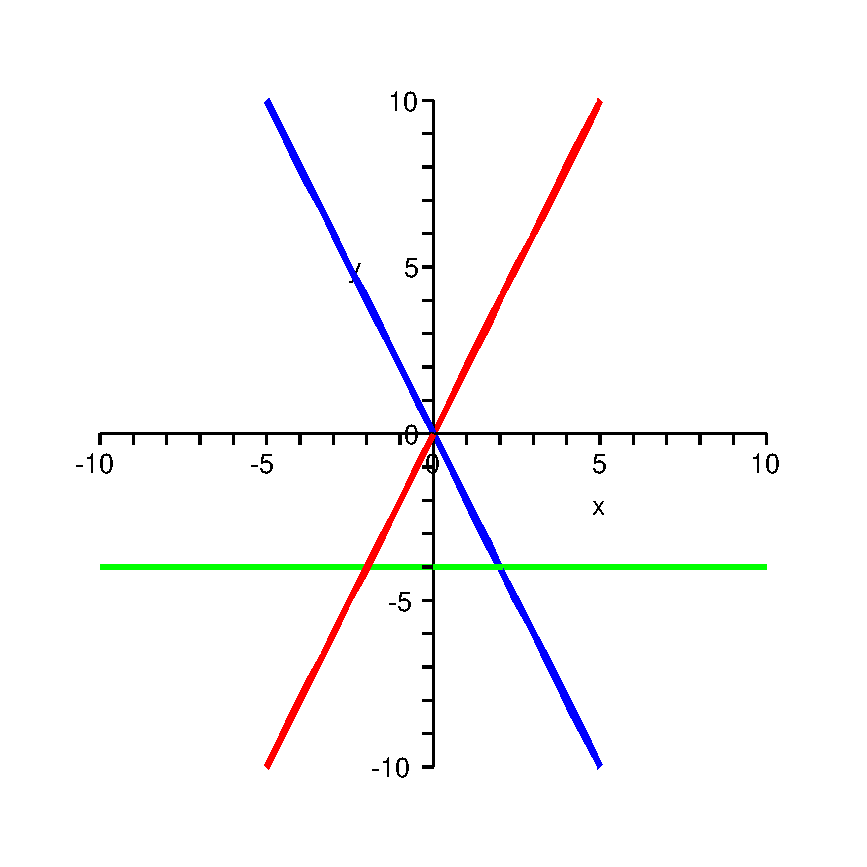
\includegraphics[width=6cm,bb=0 0 400 400]{fonction17.eps}
% fonction17.eps : 300dpi, width=3.39cm, height=3.39cm, bb=0 0 400 400
    \end{center}

The correct answer is c).\\



441-- Out of the four mathematical objects here below, which one has no dimensions?\\

a) A line\\
b) A point\\
c) A solid\\
d) A surface\\

Answer: b)\\

Explanation: \\
A point is a mathematical object with no dimensions.\\
A line is a one-dimensional mathematical object.\\
A surface is a two-dimensional mathematical object.\\
A solid is a three-dimensional mathematical object.\\
The correct answer is b).\\


451--  How many sides does an icosahedron have?\\
a) 20\\
b) 30\\
c) 40\\
d) 50\\

Answer: a)\\

Explanation: \\
An icosahedron is a 20-sided regular convex polyhedron.
The correct answer is a).
Here is an image of an icosahedron.\\
    \begin{center}
    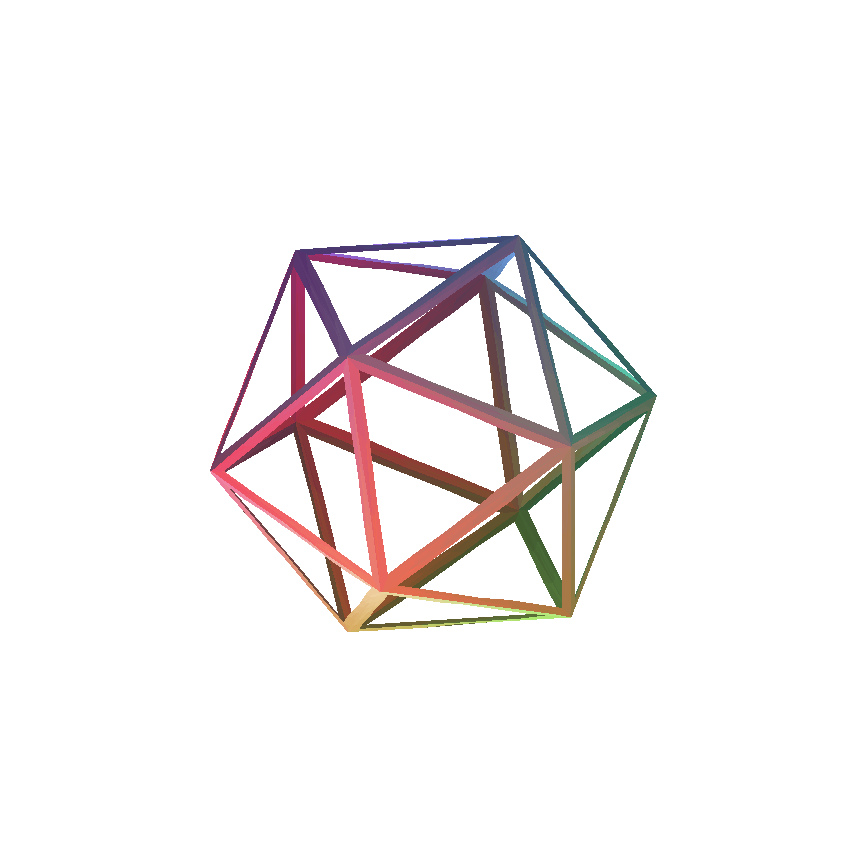
\includegraphics[width=6cm,bb=0 0 400 400]{icosaedre.eps}
% icosaedre.eps : 300dpi, width=3.39cm, height=3.39cm, bb=0 0 400 400
    \end{center}


461-- A plane cuts a cyclinder in such a way that the ending result is a circle.
What is the plane's position in relation to the cylinder?\\

a) At 45$^{\circ}$ in relation to the base\\
b) At an angle in relation to the base\\
c) Parallel to the base\\
d) Perpendicular to the base\\

Answer: c)\\

Explanation: \\
The plane must be parallel to the cylinder's base to obtain a circular section.
    \begin{center}
    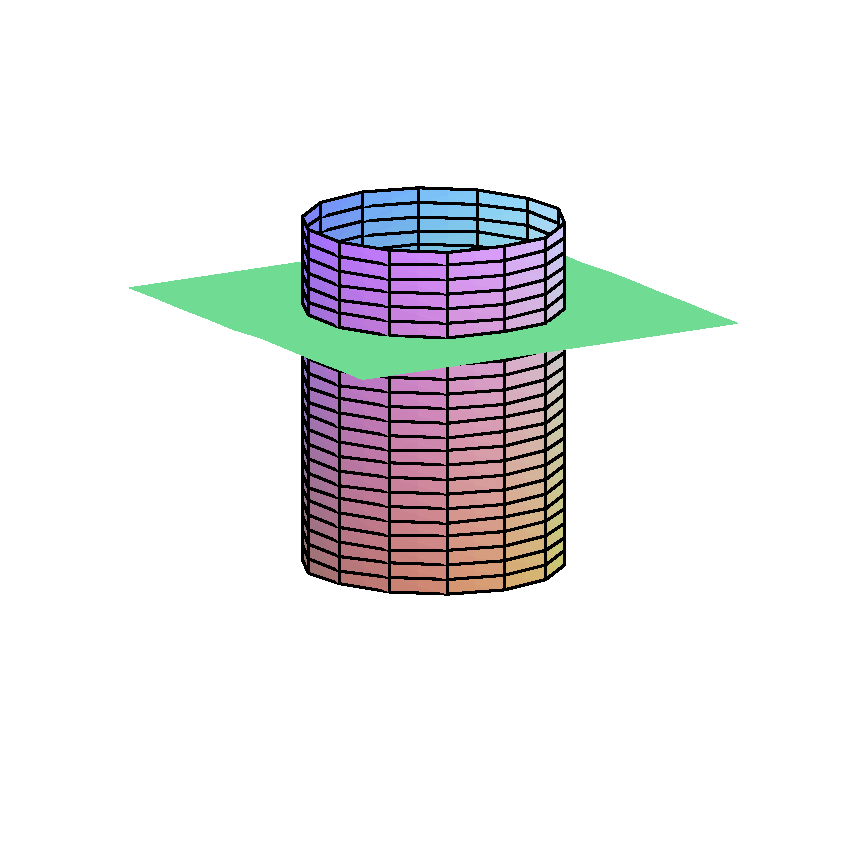
\includegraphics[width=6cm,bb=0 0 400 400]{cylplanhor.eps}
% cylplanhor.eps : 300dpi, width=3.39cm, height=3.39cm, bb=0 0 400 400
    \end{center}

The correct answer is c).\\



471-- I always have one more peak than the number of peaks that my base's polygon has.
What am I?\\

a) A cone\\
b) A prism\\
c) A pyramid\\
d) A sphere\\

Answer: c)\\

Explanation: \\
The correct answer is pyramid because the extra peak is the meeting point for each triangle forming lateral sides.
The answer is c).\\


481-- A pythagorean triplet is a triplet of whole numbers that satistfies Pythagoras' theorem.
Among the following choices, which one is a Pythagorean triplet?\\
a) (2, 4, 6)\\
b) (6, 8, 10)\\
c) (10, 12, 14)\\
d) (14, 16, 18)\\

Answer:  b)\\

Explanation: \\
A Pythagorean triplet is (6, 8, 10).\\
$a^{2}\,+\,b^{2}\,=\,c^{2}$\\
$6^{2}\,+\,8^{2}\,=\,10^{2}$\\
36 + 64 = 100\\
Thus, the correct answer is b).\\


491-- Into how many sections do two parallel planes divide up space?\\

Answer: 3\\

Explanation: \\
Space is divided up into three sections.
    \begin{center}
    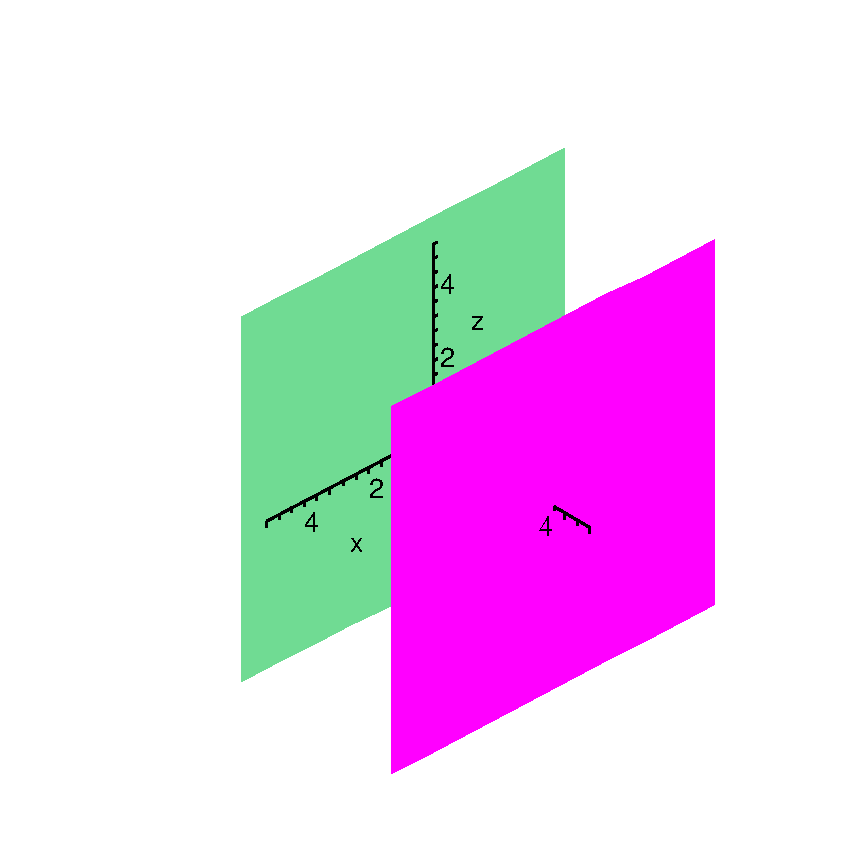
\includegraphics[width=6cm,bb=0 0 400 400]{deuplanparr.eps}
% deuplanparr.eps : 300dpi, width=3.39cm, height=3.39cm, bb=0 0 400 400
    \end{center}

The correct answer is 3.\\


501-- The sum of the length of all edges on a cube is 144 cm.
What is the volume of this cube?\\

a) 36 cm$^{3}$\\
b) 216 cm$^{3}$\\
c) 1728 cm$^{3}$\\
d) 5832 cm$^{3}$\\

Answer: c)\\

Explanation:  \\
A cube has 12 edges. Since the sum of all edges is 144 cm, each edge or side of a cube is 12 cm long.\\
Volume of a cube = $c\times c\times c$, where $c$ is the length of a side of the cube.  \\
$12^{3}=1728$\\
The cube's volume is 1728\,cm$^{3}$, thus the correct answer is c).\\


511--  Among the four isometries below, which one conserves the orientation
of the final figure in relation to the initial figure and creates parallel traces
between the two figures?\\

a) Reflection\\
b) Rotation\\
c) Sliding symetry\\
d) Translation\\

Answer: d)\\

Explanation:\\
Translation conserves the orientation of the final figure in relation to the initial figure and
creates parallel traces between these two figures.
For that reason, the correct answer is d).\\


521-- Among the four expressions here below, which one allows us to calculate a
geometric average?\\
a) $\frac{x_1\,+\,x_2\,+\,x_3\,+\,\ldots\,+\,x_n}{n}$\\[2mm]
b)
$\sqrt{\frac{x_1^{2}\,+\,x_2^{2}\,+\,x_3^{2}\,+\,\ldots\,+\,x_n^{2}}{n}}$\\[2mm]
c) $\sqrt[n]{x_1 \cdot x_2 \cdot x_3 \cdot \ldots \cdot x_n}$\\[2mm]
d)
$\frac{n}{\frac{1}{x_1}\,+\,\frac{1}{x_2}\,+\,\frac{1}{x_3}\,+\,\cdots\,+\,\frac{1}{x_n}}$\\

Answer: c)\\

Explanation: \\
Arithmetic average =
$\frac{x_1\,+\,x_2\,+\,x_3\,+\,\ldots\,+\,x_n}{n}$\\[2mm]
Quadratic average =
$\sqrt{\frac{x_1^{2}\,+\,x_2^{2}\,+\,x_3^{2}\,+\,\ldots\,+\,x_n^{2}}{n}}$\\[2mm]
Geometric average = $\sqrt[n]{x_1\cdot x_2\cdot x_3 \cdot \ldots \cdot
x_n}$\\[2mm]
Harmonic average =
$\frac{n}{\frac{1}{x_1}\,+\,\frac{1}{x_2}\,+\,\frac{1}{x_3}\,+\,\cdots\,+\,\frac{1}{x_n}}$\\[2mm]
Thus, the correct answer is c).\\



531-- Among the four choices here below, which one best describes what a median is?\\

a) A value that distributes data into two groups with exactly the same amount of numbers.
One of these groups has data smaller than the median and the other contains data that is higher than the median.\\
b) Values that distribute data into three groups with exactly the same amount of numbers.
These groups are classified in ascending order.\\
c) Values that distribute data into three groups each one with exactly the same amount of numbers.
These groups are classified in descending order.\\
d) Values that distribute data into five groups each with exactly the same amount of data.
These values are used to form five rows.\\

Answer: a) \\

Explanation: \\
A median is the value that distributes data into two groups that have the same amount of data.
The correct answer is a).\\



541-- Among the four choices here below, which one is linked to an inverse variation situation?\\

a) A curve that approaches axes without ever reaching them.\\
b) A curve that rises and falls between positive and negative values.\\
c) A straight line with a negative slope.\\
d) A straight line with a negative slope that does not pass through the origin.\\

Answer: a)

Explanation: \\
A curve that approaches axes without ever reaching them.
Here is an example of this type of graph.\\
    \begin{center}
    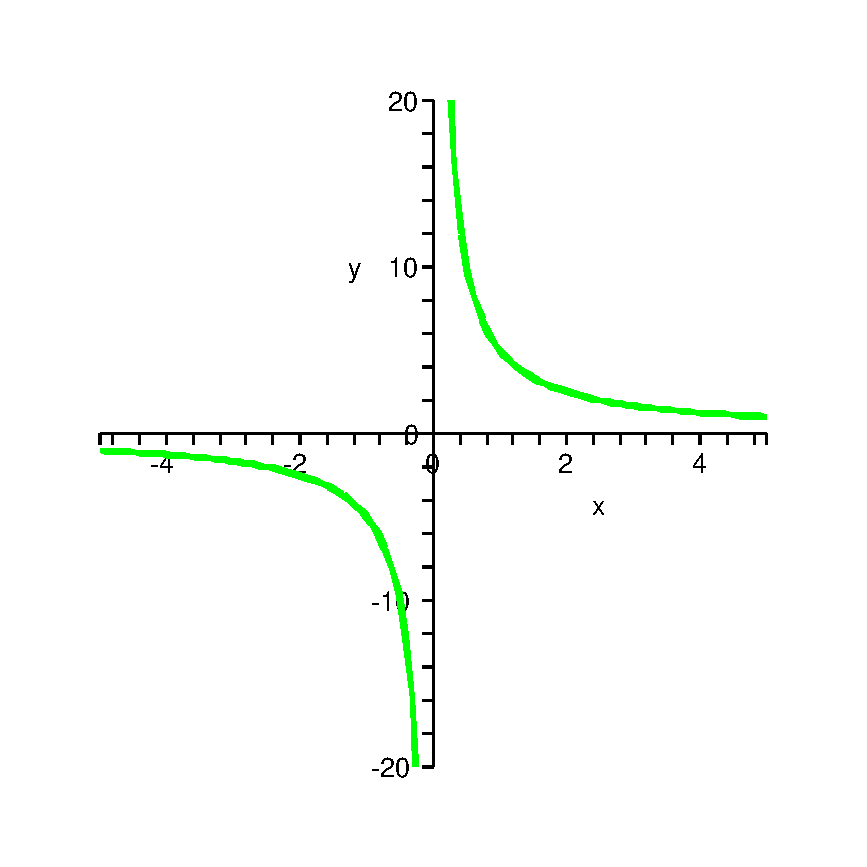
\includegraphics[width=6cm,bb=0 0 400 400]{fonction16.eps}
% fonction16.eps : 300dpi, width=3.39cm, height=3.39cm, bb=0 0 400 400
    \end{center}

The correct answer is a).\\



551-- If $x$ is the independent variable and $y$ the dependent variable,
what is the x-coordinate of the intersection of straight lines $y=6x-9$ and $y=3x\,+\,9$?\\

Answer: 6\\

Explanation: \\
Since the value of $y$ at the intersection is the same for the two straight lines, the following can be written: \\
$6x-9=3x\,+\,9$.\\
$3x-9=9$\\
$3x=18$\\
$x=6$\\
Two straight lines cross at $x=6$.\\



561-- In the right triangle ABC, segment BC is 4 cm long, segment BA 5 cm long and AC 3 cm long. The right angle is at C. Among the four choices here below, which one represents the name of the ratio $\frac{4}{5}$ in relation to angle A?\\

a) Cosine of angle A\\
b) Cotangent of angle A\\
c) Sine of angle A\\
d) Tangent of angle A\\

Answer: c)

Explanation: \\
Sine of angle A = $\frac{\textrm{length of opposite side}}{\textrm{length of hypotenuse}}\,=\,\frac{\textrm{4}}{\textrm{5}}$\\
\begin{center}
    \includegraphics[width=4.5cm]{triangle21.eps}
% triangle21.eps : 300dpi, width=3.39cm, height=3.39cm, bb=0 0 400 400
    \end{center}
The correct answer is c).\\


571-- In the triangle $ABC$, side $a$ is opposite to
angle $A$, side $b$ is opposite to angle $B$ and side $c$ is opposite to angle $C$.
Among the following four choices, which one expresses the law of sines?\\

a) $\frac{a}{\sin A}=\frac{b}{\sin B}=\frac{c}{\sin C}$\\[2mm]
b) $\frac{a}{\sin B}=\frac{b}{\sin C}=\frac{c}{\sin A}$\\[2mm]
c) $\frac{a}{\sin B}=\frac{b}{\sin A}=\frac{c}{\sin C}$\\[2mm]
d) $\frac{a}{\sin C}=\frac{b}{\sin A}=\frac{c}{\sin B}$\\

R\'eponse : a)\\

R\'etroaction : \\
The law of sines is $\frac{a}{\sin A}=\frac{b}{\sin B}=\frac{c}{\sin
C}$.\\[2mm]
Thus, the answer is a).\\


581-- Which of the following statements is true?\\

a) The repetition of several isometries is always an isometry.\\
b) The repetition of several isometries is only an isometry
if there is a composition with a translation.\\
c) The repetition of many isometries is not always an isometry.\\
d) The repetition of many isometries is never an isometry.\\

Answer: a)\\

Explanation: \\
The repetition of several isometries is always an isometry.
The correct answer is a).\\


591-- How many counterexamples are necessary to show that a statement is false?\\

a) 0\\
b) 1\\
c) 2\\
d) An infinity\\

Answer: b)\\

Explanation: \\
Only one counterexample is enough to prove a statement to be false.
The correct answer is b).\\



601-- Among the four examples here below, which one is true?\\

a) Two triangles are congruent when their three corresponding angles are congruent.\\
b) Two triangles are the same colour when their three corresponding angles are congruent.\\
c) Two triangles are identical when their three corresponding angles are congruent.\\
d) Two triangles are similar when their three corresponding angles are congruent.\\

Answer: d) \\

Explanation: \\
Two triangles are similar when their three counterpart angles are congruent.   \begin{center}
    \includegraphics[height=3.39cm]{601.eps}
% napperon.eps : 300dpi, width=3.39cm, height=3.39cm, bb=0 0 400 400
    \end{center}  The correct answer is d).\\


611-- Which of the following four statements is true?\\

a) The total area ratio of two similar solids is half of the
similarity ratio of the two solids.\\
b) The total area ratio of two similar solids is equal to the similarity ratio
between two solids.\\
c) The total area ratio of two similar solids is equal to the square of the similarity
ratio between the two solids.\\
d) The total area ratio of two similar solids is equal to the cube of the similarity ratio between the two solids.\\

Answer: c)\\

Explanation: \\
The total area ratio of two similar solids is equal to the square of the similarity ratio between the two solids.
Thus, the answer is c).\\

\end{document}
